% Adjust these for the path of the theme and its graphics, relative to this file
%\usepackage{beamerthemeFalmouthGamesAcademy}
\usepackage{../../beamerthemeFalmouthGamesAcademy}
\usepackage{multimedia}
\usepackage{soul}
\usepackage{tikz}
\usepackage{verbatim}
\graphicspath{ {../../} }
\usepackage{csquotes}
\usepackage{hyperref}
\hypersetup{
    colorlinks=true,
    linkcolor=blue,
    filecolor=magenta,      
    urlcolor=cyan,
}

% Default language for code listings
\lstset{language=C++,
        morekeywords={each,in,nullptr}
}

% For strikethrough effect
\usepackage[normalem]{ulem}
\usepackage{wasysym}

\usepackage{pdfpages}

% http://www.texample.net/tikz/examples/state-machine/
\usetikzlibrary{arrows,automata}

\newcommand{\modulecode}{COMP260}\newcommand{\moduletitle}{Distributed Systems}\newcommand{\sessionnumber}{5}

\begin{document}
\title{\sessionnumber: \normalsize{Human-Centred Design(HCI)}}
\subtitle{\modulecode: \moduletitle}

\frame{\titlepage} 

% ATTENDANCE
\begin{frame}
	\frametitle{Sign the Register}
	\begin{figure}
		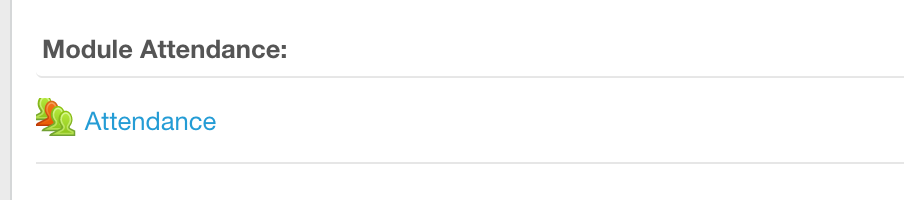
\includegraphics[scale=.5]{assets/attendance}
		\caption{\tiny{http://learningspace.falmouth.ac.uk/course/view.php?id=1254\&section=1 }}
	\end{figure}
\end{frame}

% MODULE ROADMAP
\begin{frame}
	\frametitle{Module Roadmap}
	\begin{figure}
		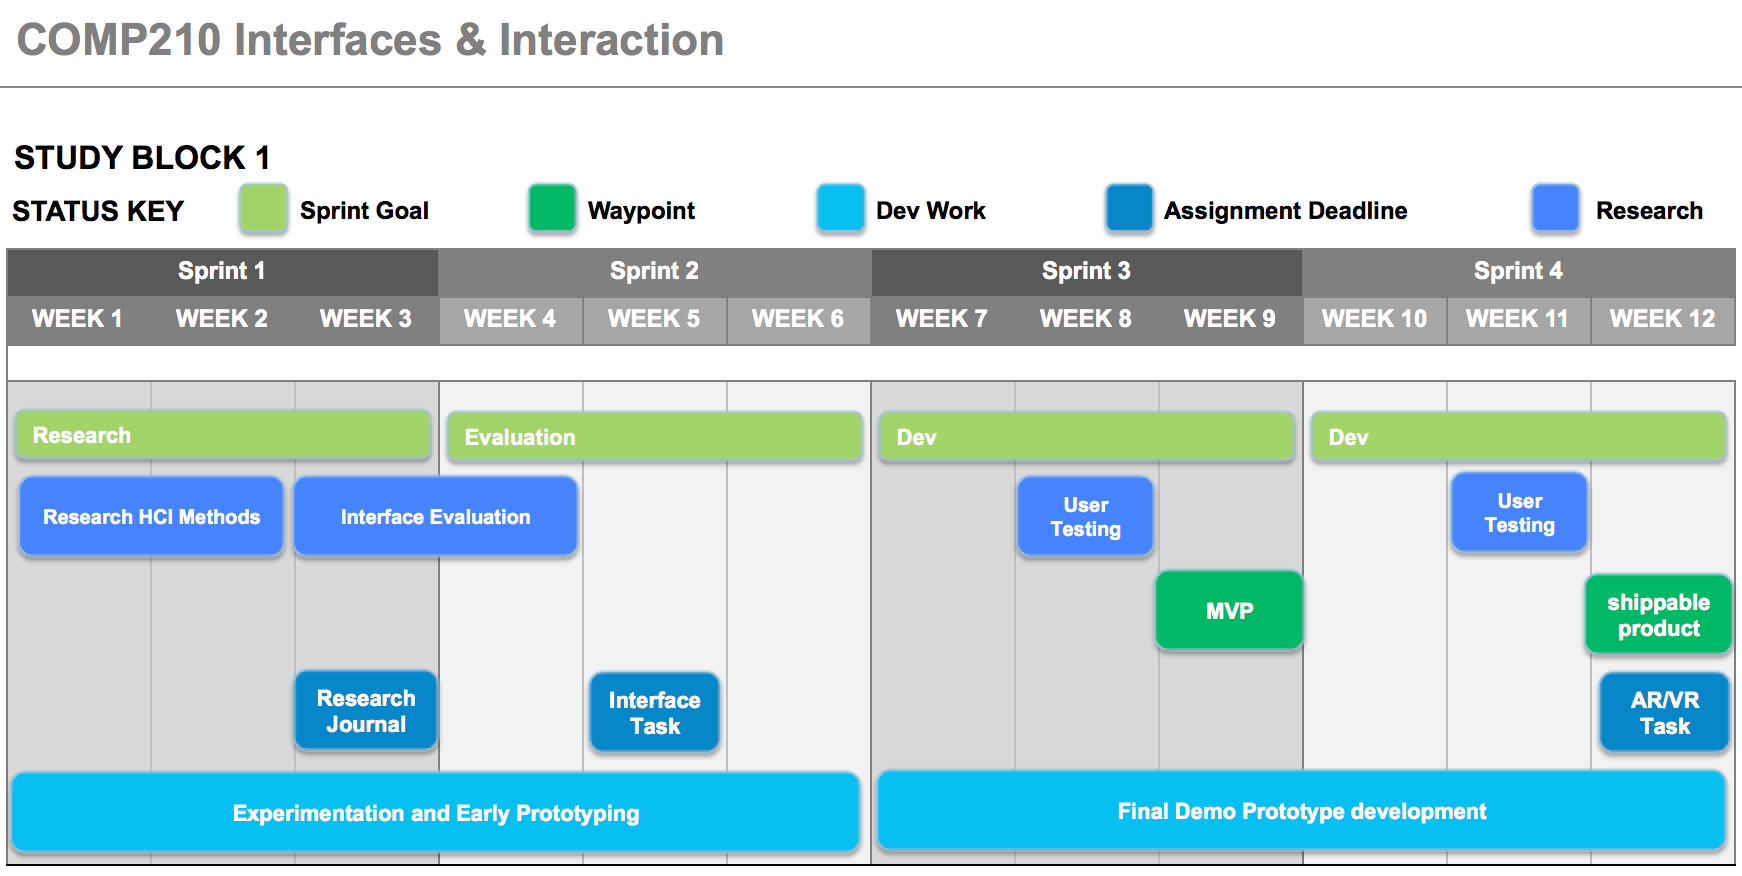
\includegraphics[scale=.36]{assets/roadmap}
	\end{figure}
\end{frame}


% ASSIGNMENT BRIEFS
\begin{frame}
	\frametitle{Assignment Briefs}
	\begin{itemize}
		\item \textbf{Produce} a journal detailing your research into HCI research
		\item \textbf{Evaluate} an existing screen-based game interface
		\item \textbf{Design} and \textbf{develop} an interface that incorporates either AR or VR
	\end{itemize}
\end{frame}

% LEARNING OUTCOMES
\begin{frame}
	\frametitle{Learning Outcomes }
	
	\begin{itemize}
		\item \textbf{Explain} what is meant by the term human-computer interaction (HCI)
		\item \textbf{Discuss} how HCI has changed over the years
		\item \textbf{Outline} some basic HCI principles as described by Don Norman in his book, The Design of Everyday Things  
	\end{itemize}
\end{frame}

\begin{frame}
	\frametitle{Human-Computer Interaction}
	''If we didn't have people, everything would work so much better`` Donald A. Norman
	
	\begin{center}
		\huge what is HCI?
	\end{center}
\end{frame}

\begin{frame}
	\begin{center}
	HCI is the study of the relationship between people and technology
	\end{center}
	\begin{figure}
		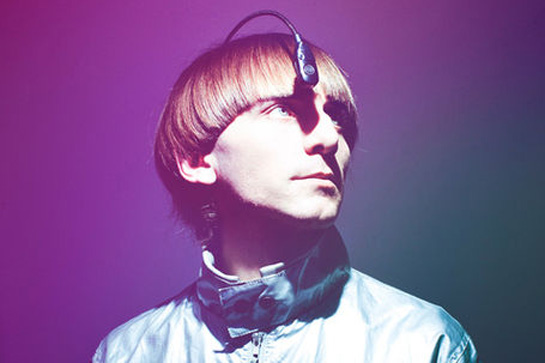
\includegraphics[scale=.45]{assets/cyborgist}
		\caption{\href{https://www.youtube.com/watch?v=C_OnYqx3ynA}{Cyborg Neil Harbisson} with his antenna implant}
	\end{figure}
\end{frame}

\begin{frame}
	\frametitle{A Little Bit of History}
	\begin{itemize}
		\item Commonly understood that HCI formally acknowledged as a field of study in1982
		\item driven by the shift from secure cool room computers to personal computer - Apple 2 IBM PC Commodore
		\item In essence, non-engineers having access to computers
		\item Early computers were pretty daunting to non-engineers
		\item HCI was born from the shift from specialist users to day-to-day use by non-engineers
	\end{itemize}
\end{frame}

\begin{frame}
	\frametitle{Ivan Sutherland}
	\begin{figure}
		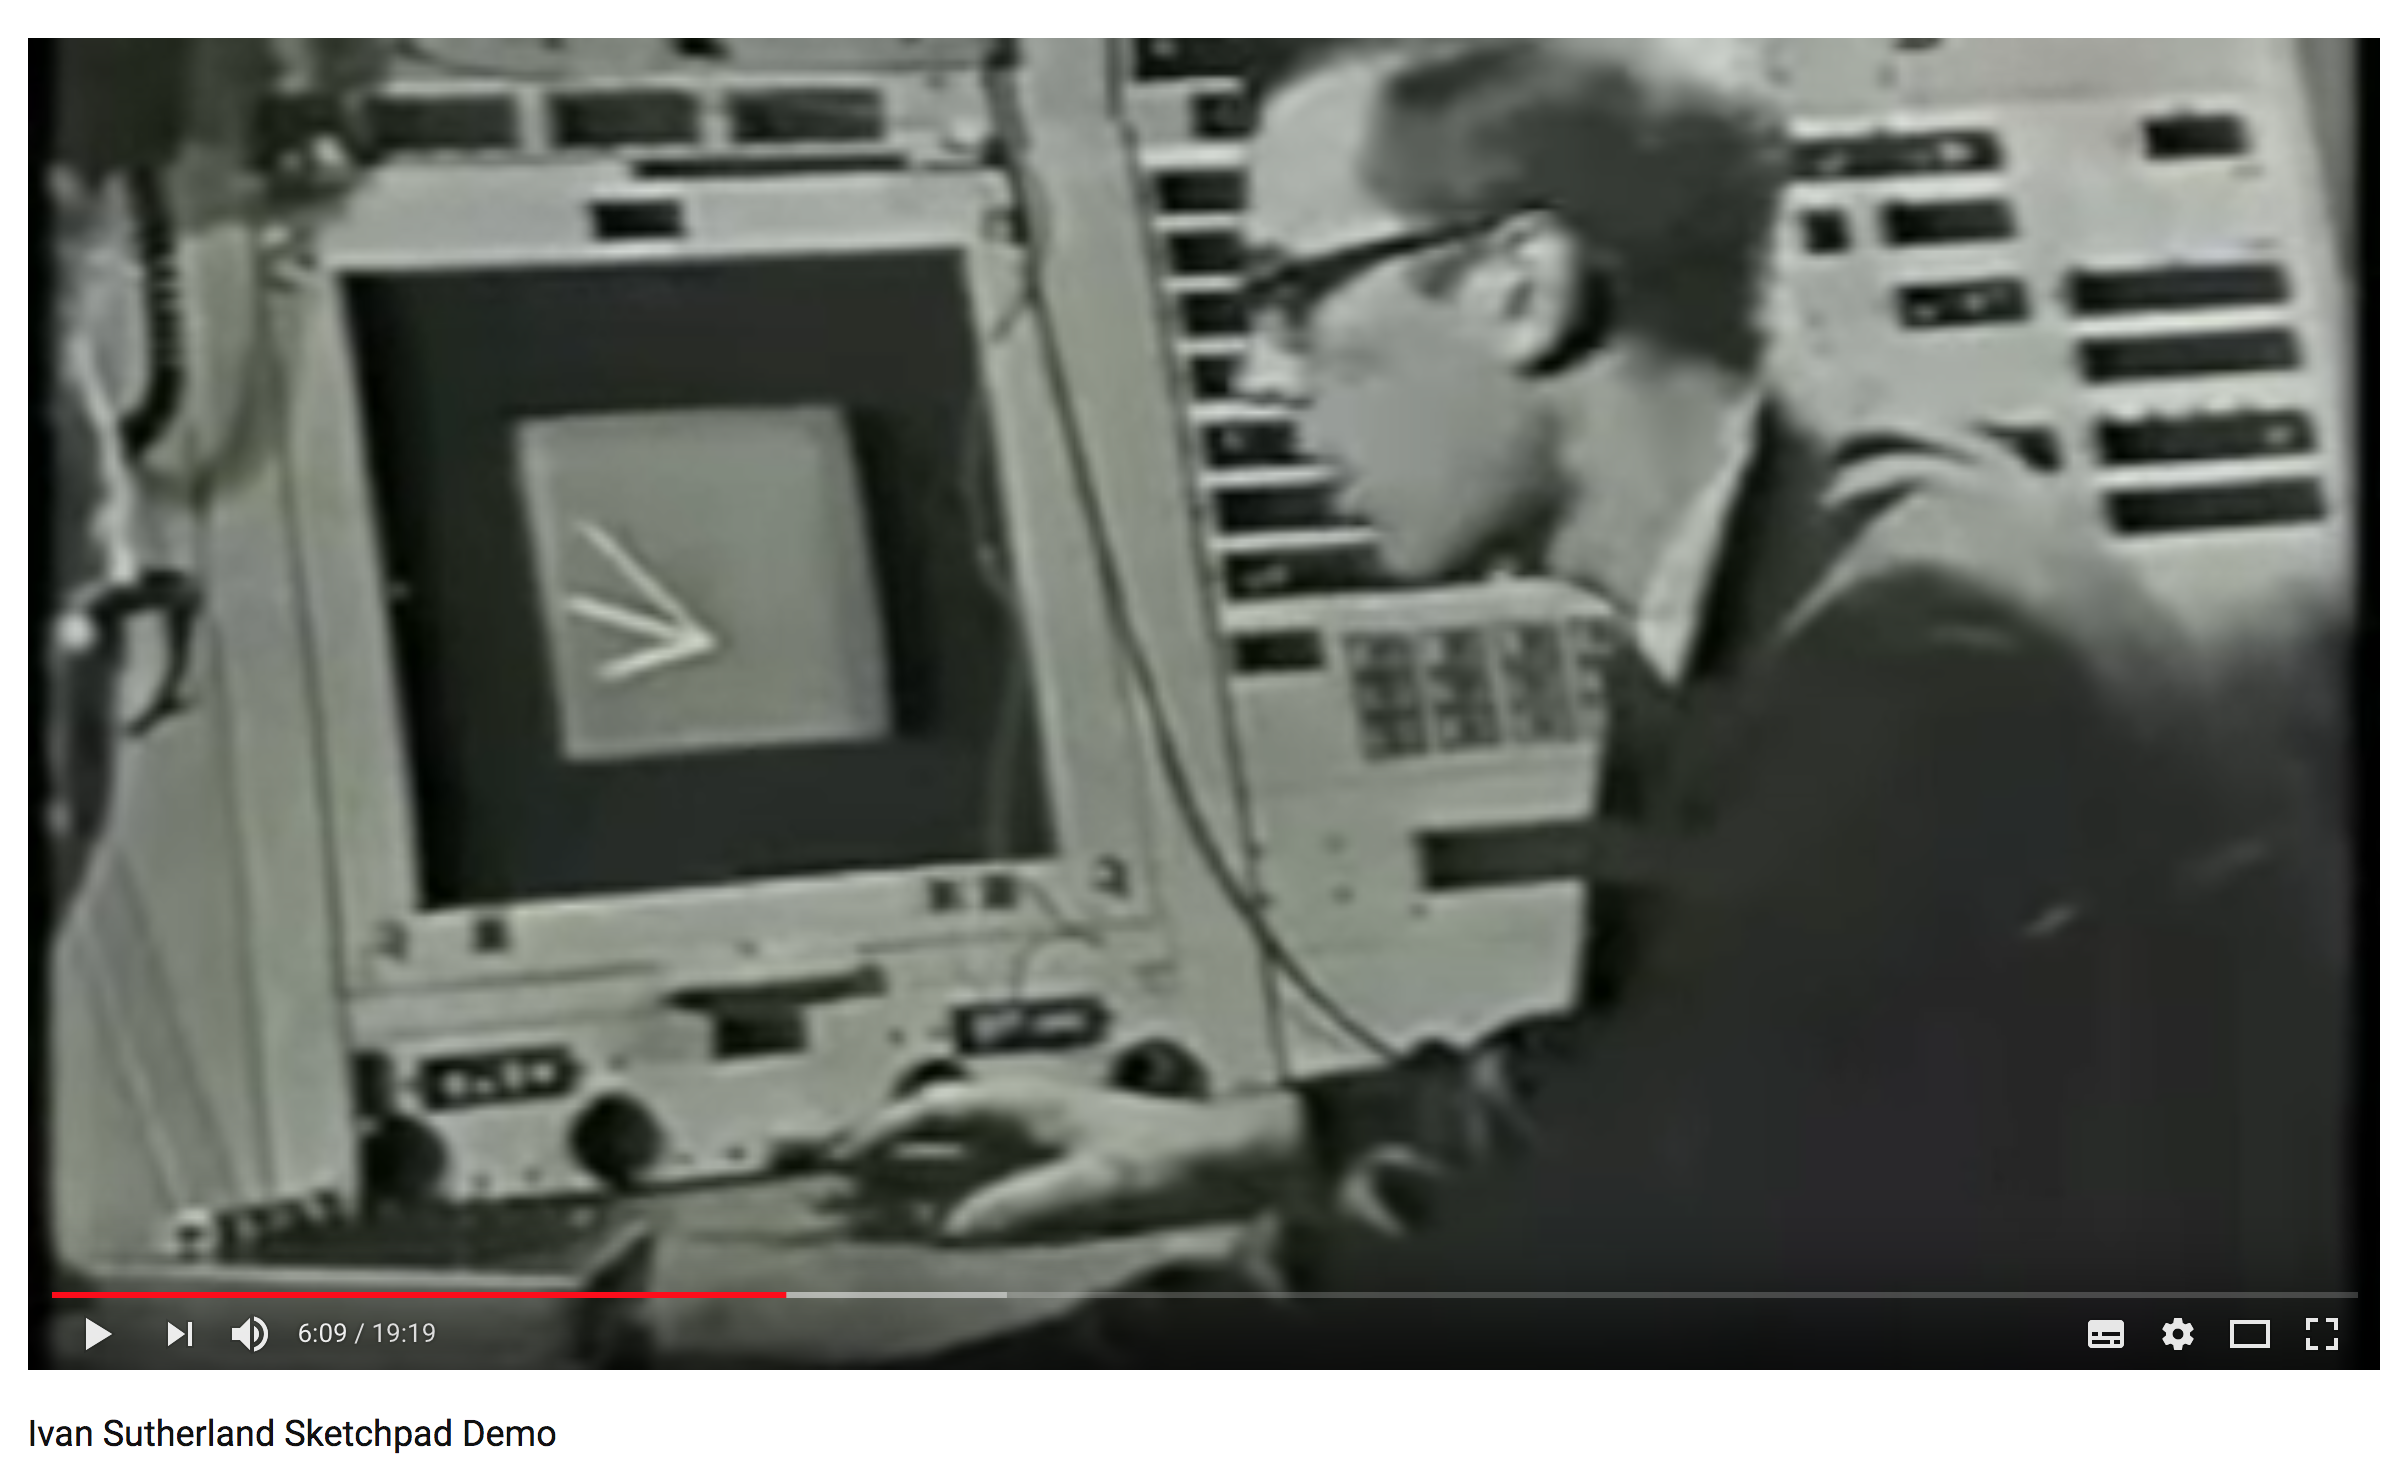
\includegraphics[scale=.2]{assets/sutherland}
		\caption{\href{https://youtu.be/6orsmFndx_o?t=655}{Youtube link for Sketchpad demo filmed in the early 60s}}
	\end{figure}
\end{frame}

\begin{frame}
	\frametitle{More recently...}
	\begin{center}
		Early 90s HCI blew up as the internet and web went mainstream and there was an explosion of new interface and communication methods
	\end{center}
	\textbf{Other Notable Shifts: }
	
	\begin{center}
		Fixed computers\textless 2004\textgreater  portable devices \\ ~ \\
                    Authored content\textless 2004\textgreater  user generated content
         \end{center}
\end{frame}

\begin{frame}
	\frametitle{NOW}
	\begin{center}
		Tech Buzzword Bingo!
	\end{center}
	\begin{itemize}
		\item Mobile
		\item Multitouch
		\item Gestures and natural computing
		\item Sensors
		\item Embedded
		\item Wearables
		\item Sustainability
		\item Big Data
		\item Social computing
		\item Accessibility
		\item Mixed Reality
	\end{itemize}
\end{frame}

\begin{frame}
	Lets begin with the principle that all artificial things are designed. \\ ~ \\
	
	Who is doing the designing?
	\begin{center}
		\pause Are you doing any design? 
	\end{center}
\end{frame}

\begin{frame}
	\frametitle{HCI - A Crash Course}
	\begin{center}
		\huge Do not...
	\end{center}
	\begin{itemize}
		\item Presume prior knowledge of the audience
		\item Especially, if they are a similar demographic to you
		\item Expect people to read the instructions
		\item Blame the user for errors
		\item Get frustrated with the user for unpredictable behaviour
	\end{itemize}
\end{frame}

\begin{frame}
	\frametitle{HCI is complex because...}
	\begin{itemize}
		\item Borrow methods from other fields
		\item Create standards derived from other fields
		\item Involves Humans
	\end{itemize}
\end{frame}

\begin{frame}
	\begin{center}
		If HCI is the study of the relationship between people and technology what fields might that span?
	\end{center}
	\pause
	\begin{itemize}
		\item Computer Science (duh)
		\item Sociology
		\item Psychology
		\item Communication
		\item Human factors engineering
		\item Industrial engineering
		\item rehabilitation engineering
		\item and many more.
	\end{itemize}	
\end{frame}

\begin{frame}
	\frametitle{HCI Research}
	\begin{displayquote}	
		``HCI research requires both rigorous methods and relevance'' \\ ~ \\ - Donald A. Norman
	\end{displayquote} 
	\pause
	
	
	We use it to influence interface design, development process, user training, and public policy. \\ ~ \\
	Generally, to improve our relationship with computers.

\end{frame}

\begin{frame}
		
	\frametitle{What can be considered HCI contributions?}

	\begin{itemize}
		\item Empirical
		\item Artefact
		\item Methodological
		\item Dataset
		\item Survey	
		\item Opinion
		\item theoretical
	\end{itemize}

	\href{http://interactions.acm.org/archive/view/may-june-2016/research-contribution-in-human-computer-interaction}{(Source)} 
\end{frame}

\begin{frame}
	\frametitle{These are Exciting Times}
	\begin{itemize}
		\item Tools are much better now
		\item Eye tracking, sensors (EMG EEG)
		\item Access to the masses - mechanical Turk, social networks, large amounts of generated content to analyse
		\item Automation - AI machine learning, neural networks
	\end{itemize}
\end{frame}

\begin{frame}
	\frametitle{Donald Norman}
	\begin{figure}
		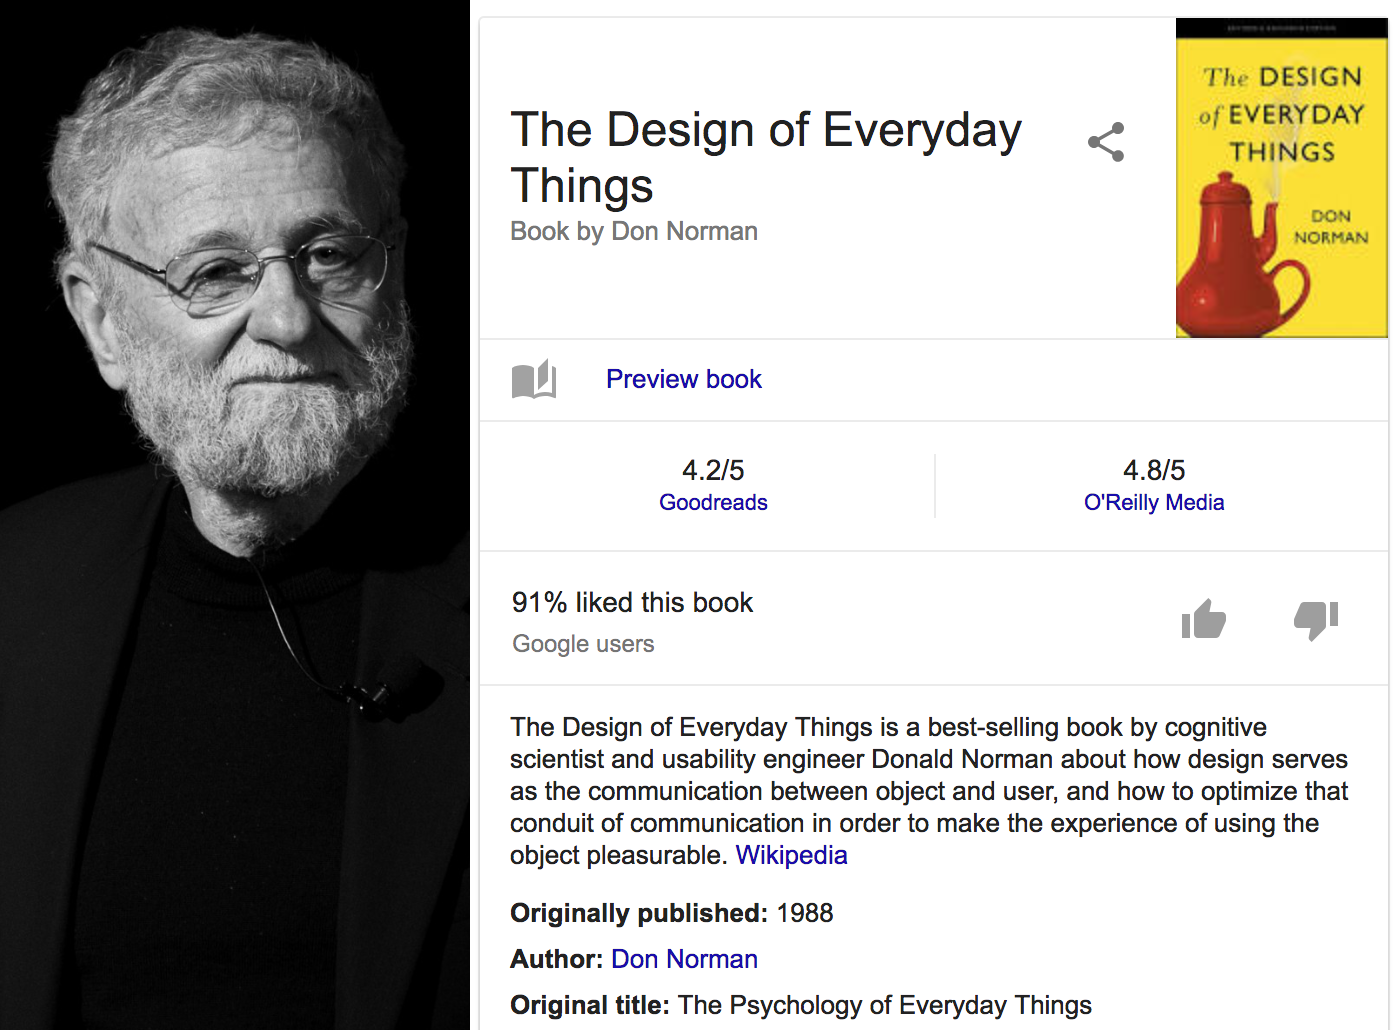
\includegraphics[scale=.2]{assets/don}
	\end{figure}
\end{frame}

\begin{frame}
	\frametitle{Affordances}
	\begin{itemize}
		\item Standard Affordances
		\item Perceivable Affordances
		\item Anti-Affordances
	\end{itemize}
\end{frame}

\begin{frame}
	\begin{center}
		\huge Signifiers
	\end{center}
\end{frame}

\begin{frame}
	\begin{center}
		\huge Mappings
	\end{center}
\end{frame}

\begin{frame}
	\begin{center}
		\huge Mental models
	\end{center}
\end{frame}



\begin{frame}
	\frametitle{\href{https://www.nngroup.com/}{Nielsen Norman Group}}
	\begin{figure}
		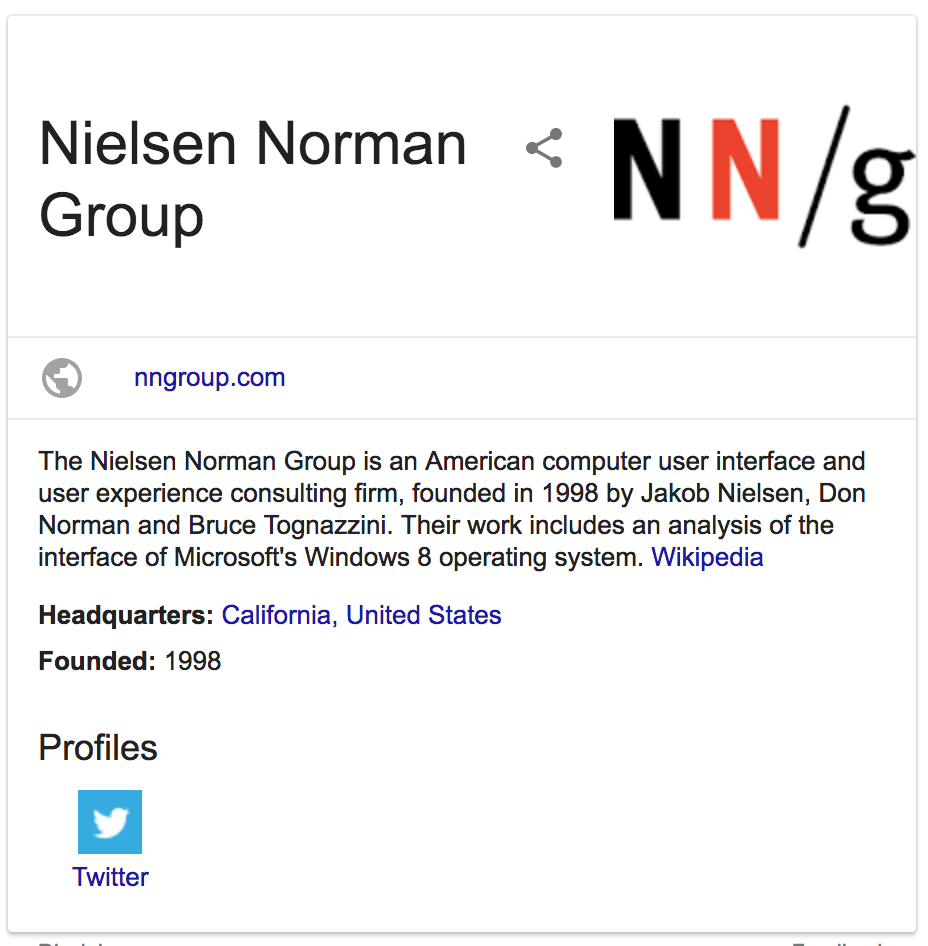
\includegraphics[scale=.35]{assets/nngroup}
	\end{figure}
\end{frame}



\end{document}
